\documentclass{standalone}

\usepackage{amsmath,amsfonts,amssymb,amsthm,mathtools} 
\usepackage{fontspec}            % пакет для подгрузки шрифтов
\setmainfont{Amiri}   % задаёт основной шрифт документа

% why do we need \newfontfamily:
% http://tex.stackexchange.com/questions/91507/
\newfontfamily{\cyrillicfonttt}{Amiri}
\newfontfamily{\cyrillicfont}{Amiri}
\newfontfamily{\cyrillicfontsf}{Burst My Bubble}
% Иногда тех не видит структуры шрифтов. Эти трое бравых парней спасают ситуацию и доопределяют те куски, которые Тех не увидел.

\usepackage{unicode-math}     % пакет для установки математического шрифта
\setmathfont{Asana Math}      % шрифт для математики

\usepackage{polyglossia}      % Пакет, который позволяет подгружать русские буквы
\setdefaultlanguage{russian}  % Основной язык документа
\setotherlanguage{english}    % Второстепенный язык документа

\usepackage{pgf,tikz,pgfplots}
\usetikzlibrary{arrows,calc}
\usepackage{relsize} 

\usepackage{graphicx} 
\usepackage{rotating}
\usepackage{xcolor}
\usepackage{color}

\newcommand{\BBig}{\fontsize{60}{60}\selectfont}

\definecolor{bl}{HTML}{333333}
\definecolor{latxlatx}{HTML}{434545}


\begin{document}

\centering

\begin{tikzpicture}[
        scale=2,
        dot/.style={circle,fill=black,minimum size=4pt,inner sep=0pt,
            outer sep=-1pt},
    ]

% picture with lion 
\node[inner sep=0pt] (russell) at (0,0.55){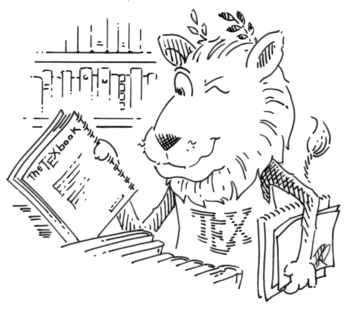
\includegraphics[angle=0,scale=0.4]{lion.png}};       
    
\begin{scope}[rotate=30]     
% Radius of regular polygons
  \newdimen\R
  \R=2cm
  \coordinate (center) at (0,0);
 \draw (0:\R)
     \foreach \x in {60,120,...,360} {  -- (\x:\R) }
              -- cycle (300:\R)
              -- cycle (240:\R)
              -- cycle (180:\R)
              -- cycle (120:\R)
              -- cycle (60:\R)
              -- cycle (0:\R)  [line width=1.9mm,color=latxlatx,fill=gray,fill opacity=0];
\end{scope}
% fill

  
% tex logo          
\draw[color=black,draw,align=left] (-1.1,-1) node[right] {{\color{latxlatx} \BBig \LaTeX}};                           
\end{tikzpicture}


%\begin{tikzpicture}[scale=2]
%
%% Radius of regular polygons
%  \newdimen\R
%  \R=2cm
%  \coordinate (center) at (0,0);
% \draw (0:\R)
%     \foreach \x in {60,120,...,360} {  -- (\x:\R) }
%              -- cycle (300:\R)
%              -- cycle (240:\R)
%              -- cycle (180:\R)
%              -- cycle (120:\R)
%              -- cycle (60:\R)
%              -- cycle (0:\R)  [line width=3.2pt,color=gray,fill=white,fill opacity=0.1];
%       
%% picture with R-emblem
%    \node[inner sep=0pt] (russell) at (0,0)
%    {
\includegraphics[angle=0,scale=0.1]{RStudio-Ball.png}};                                  
%\end{tikzpicture}

\end{document}
